% Latex template: mahmoud.s.fahmy@students.kasralainy.edu.eg
% For more details: https://www.sharelatex.com/learn/Beamer

\documentclass[usenames,dvipsnames]{beamer}

\usepackage[english]{babel}				% Set language
\usepackage[utf8x]{inputenc}
\usepackage[round]{natbib}
\usepackage{multirow}
\usepackage{tikz}
\usepackage{multicol}
\usepackage[most]{tcolorbox}
\usepackage{framed, color}
\usepackage{cancel}
\usepackage{comment}
\usetikzlibrary{calc}
\usepackage[normalem]{ulem}
\usetheme{Frankfurt}
\usepackage{xcolor}
\usepackage{natbib}
\usepackage{pifont}
\usepackage{amsmath}
\usepackage{amssymb}% http://ctan.org/pkg/amssymb
\usepackage{color}

\newcommand{\xmark}{\ding{55}}%

\newcommand{\greencheck}{{\color{Green}\boldsymbol{\checkmark}}}

\definecolor{darkorchid}{rgb}{0.6, 0.2, 0.8}


\makeatletter
\long\def\beamer@@ssection*#1{\beamer@section[]{}}

\setbeamertemplate{frametitle continuation}{(\insertcontinuationcountroman)}

\makeatother

\newcommand{\bstau}{\boldsymbol{\tau}}
\newcommand{\hbstau}{\boldsymbol{\hat \tau}}
\newcommand{\taur}{\boldsymbol{\hat \tau_r}}
\newcommand{\htaur}{\boldsymbol{\hat \tau_r}}
\newcommand{\tauo}{\boldsymbol{\hat \tau_o}}
\newcommand{\htauo}{\boldsymbol{\hat \tau_o}}
\newcommand{\htauw}{\boldsymbol{\hat \tau_w}}
\newcommand{\bst}{\boldsymbol{\theta}}
\newcommand{\bsxi}{\boldsymbol{\xi}}
\newcommand{\bsD}{\boldsymbol{W}}
\newcommand{\bsnu}{\boldsymbol \nu}


\newcommand{\bspsi}{\boldsymbol{\hat \psi}}
\newcommand{\bsSig}{\boldsymbol{\Sigma}}
\newcommand{\bsp}{\boldsymbol{ \hat \psi}}

\newcommand{\hbsSig}{\boldsymbol{\hat \Sigma}}
\newcommand{\ident}{\boldsymbol{I}}
\newcommand{\bsdelt}{\boldsymbol{\delta}}
\newcommand{\hbsdelt}{\boldsymbol{\hat \delta}}
\newcommand{\bskap}{\boldsymbol{ \kappa}}
\newcommand{\hbskap}{\boldsymbol{ \hat \kappa}}



\newcommand{\OR}{\text{OR}}
\newcommand{\Conv}{\text{Conv}}
\newcommand{\Ext}{\text{Ext}}
\newcommand{\Ell}{\text{Ell}}
\newcommand{\bsv}{\boldsymbol{v}}

\newcommand{\Tr}{\text{Tr}}
\newcommand{\Var}{\text{Var}}
\newcommand{\URE}{\text{URE}}
\newcommand{\E}{\mathbb{E}}

\newcommand{\tauu}{\boldsymbol{\hat \tau_r}}
\newcommand{\taub}{\boldsymbol{\hat \tau_o}}
\newcommand{\tauuk}{\hat \tau_{rk}}
\newcommand{\taubk}{\hat \tau_{ok}}

\newcommand{\gammamm}{\hat \gamma_{\text{mm}}^2}
\newcommand{\etamm}{\hat \eta_{\text{mm}}^2}

\newcommand{\gammammone}{\hat \gamma_{\text{mm,1}}^2}
\newcommand{\etammone}{\hat \eta_{\text{mm,1}}^2}

\newcommand{\gammammtwo}{\hat \gamma_{\text{mm,2}}^2}
\newcommand{\etammtwo}{\hat \eta_{\text{mm,2}}^2}


\newcommand{\gammamle}{\hat \gamma_{\text{mle}}^2}
\newcommand{\etamle}{\hat \eta_{\text{mle}}^2}

\newcommand{\ure}{\text{URE}}
\newcommand{\gammaure}{\hat \gamma_{\text{ure}}^2}
\newcommand{\etaure}{\hat \eta_{\text{ure}}^2}

\newcommand{\bspmm}{\boldsymbol{\hat \psi_{\textbf{mm}}}}
\newcommand{\bspmmone}{\boldsymbol{\hat \psi_{\textbf{mm,1}}}}
\newcommand{\bspmmtwo}{\boldsymbol{\hat \psi_{\textbf{mm,2}}}}
\newcommand{\bspmle}{\boldsymbol{\hat \psi_{\textbf{mle}}}}
\newcommand{\bspure}{\boldsymbol{\hat \psi_{\textbf{ure}}}}
\newcommand{\tauw}{\boldsymbol{\hat \tau_w}}



\newcommand\phz{\phantom{0}}

%\let\oldcite=\cite                                                              
% \renewcommand{\cite}[1]{\textcolor[rgb]{.3,.3,.8}{\oldcite{#1}}}

\let\oldcite=\cite
\let\oldcitep=\citep 
\renewcommand{\cite}[1]{\textcolor[rgb]{.3,.3,.8}{\oldcite{#1}}}
\renewcommand{\citep}[1]{\textcolor[rgb]{.3,.3,.8}{\oldcitep{#1}}}

% Uncomment this to have the outline at the beginning of each section highlighted.
\AtBeginSection[]
{
  \begin{frame}{Outline}
    \tableofcontents[currentsection]
    \end{frame}
}
   
\AtBeginSubsection[]
{
  \begin{frame}{Outline}
    \tableofcontents[currentsection]
    \end{frame}
}
   



\mode<presentation>						% Set options
{
  \usetheme{default}					% Set theme
  \usecolortheme{default} 				% Set colors
  \usefonttheme{default}  				% Set font theme
  \setbeamertemplate{caption}[numbered]	% Set caption to be numbered
}

% Uncomment this to have the outline at the beginning of each section highlighted.
%\AtBeginSection[]
%{
%  \begin{frame}{Outline}
%    \tableofcontents[currentsection]
%  \end{frame}
%}

\usepackage{graphicx}					% For including figures
\usepackage{booktabs}					% For table rules
\usepackage{hyperref}					% For cross-referencing
\definecolor{shadecolor}{rgb}{1, 0.8, 0.3}

\title{Shrinkage Estimation for Causal Inference and Experimental Design}	% Presentation title
\author{\textbf{Evan T. R. Rosenman}$^{\dag}$, Guillaume Basse, Mike Baiocchi,\\ Art B. Owen, Francesca Dominici, and Luke Miratrix}								% Presentation author
\institute{$^{\dag}$ Assistant Professor, Claremont McKenna College}					% Author affiliation
\date{September 16, 2023}									% Today's date	
								% Today's date	


\newcommand{\wh}{\widehat}
\newcommand{\wt}{\widetilde}
\newcommand{\real}{\mathbb{R}}

\newcommand{\tikzmark}[1]{\tikz[overlay,remember picture] \node (#1) {};}
\newtcolorbox{mybox}[2][]{colback=blue!5!white,colframe=blue!75!black,fonttitle=\bfseries, title=#2,#1}

\newcommand{\bsx}{\boldsymbol{x}}
\newcommand{\bsy}{\boldsymbol{y}}

\newcommand{\bsX}{\boldsymbol{X}}

\newcommand{\e}{\mathbb{E}}
\newcommand{\var}{\mathrm{var}}
\newcommand{\cov}{\mathrm{cov}}

\newcommand{\rct}{\mathcal{R}}
\newcommand{\odb}{\mathcal{O}}

\newcommand{\err}{\varepsilon}

\renewcommand{\le}{\leqslant}
\renewcommand{\ge}{\geqslant}

\newcommand{\tran}{\mathsf{T}}

\newcommand{\simiid}{\stackrel{\mathrm{iid}}\sim}

\newcommand{\rd}{\,\mathrm d}

\newcommand{\one}{\boldsymbol{1}}
\DeclareMathOperator*{\argmin}{argmin}

% Specialized notation for this paper.
% Fiddly notation seems to require copious definitions, some for purely carpal reasons.
% Small roman subscripts are more readable than smal italic ones.
% There are several \renewcommands that might be problematic later.

\newcommand{\edelt}{\e_{\delta}}   % Delta method mean, we might have to switch notation later
\newcommand{\vdelt}{\var_{\delta}} 
\newcommand{\bdelt}{\bias_{\delta}} 

\renewcommand{\k}{\mathrm{k}}
\renewcommand{\r}{\mathrm{r}}
\newcommand{\s}{\mathrm{s}}
\renewcommand{\o}{\mathrm{o}}

\newcommand{\rk}{\mathrm{rk}}
\newcommand{\rkt}{\mathrm{rkt}}
\newcommand{\rkc}{\mathrm{rkc}}

\newcommand{\rt}{\mathrm{rt}}
\newcommand{\rc}{\mathrm{rc}}

\newcommand{\ok}{\mathrm{ok}}
\newcommand{\okt}{\mathrm{okt}}
\newcommand{\okc}{\mathrm{okc}}

\newcommand{\ot}{\mathrm{ot}}
\newcommand{\oc}{\mathrm{oc}}

\newcommand{\kt}{\mathrm{kt}}
\newcommand{\kc}{\mathrm{kc}}

\renewcommand{\it}{it}
\newcommand{\ic}{ic}
\newcommand{\ip}{i'}
\newcommand{\itp}{i't}

\newcommand{\sk}{sk}
\newcommand{\skt}{\mathrm{skt}}
\newcommand{\skc}{\mathrm{skc}}

\newcommand{\st}{\mathrm{st}}
\renewcommand{\sc}{\mathrm{sc}}


\newcommand{\nrk}{n_{\rk}}
\newcommand{\nrkt}{N_{\rkt}}
\newcommand{\nrkc}{N_{\rkc}}

\newcommand{\nrt}{n_{\rt}}
\newcommand{\nrc}{n_{\rc}}


\newcommand{\no}{n_{\o}}
\newcommand{\nok}{n_{\ok}}
\newcommand{\nokt}{N_{\okt}}
\newcommand{\nokc}{N_{\okc}}

\newcommand{\fr}{f_{\r}}
\newcommand{\fo}{f_{\o}}

\newcommand{\byr}{\bar Y_{\r}}
\newcommand{\byrk}{\bar Y_{\rk}}
\newcommand{\byrkt}{\bar Y_{\rkt}}
\newcommand{\byrkc}{\bar Y_{\rkc}}

\newcommand{\byrt}{\bar Y_{\rt}}
\newcommand{\byrc}{\bar Y_{\rc}}

\newcommand{\byo}{\bar Y_{\o}}
\newcommand{\byok}{\bar Y_{\ok}}
\newcommand{\byokt}{\bar Y_{\okt}}
\newcommand{\byokc}{\bar Y_{\okc}}

\newcommand{\yit}{Y_{i}(1)}
\newcommand{\yic}{Y_{i}(0)}

\newcommand{\yitp}{Y_{\itp}}

\newcommand{\wi}{W_i}
\newcommand{\wit}{W_{i}}
\newcommand{\wic}{(1-W_{i})}

\newcommand{\witp}{W_{\itp}}


\newcommand{\sok}{S_{\ok}}
\newcommand{\sokt}{S_{\okt}}
\newcommand{\sokc}{S_{\okc}}
\newcommand{\soktc}{S_{\mathrm{oktc}}}

\newcommand{\sr}{S_{\r}}
\newcommand{\srt}{S_{\rt}}
\newcommand{\src}{S_{\rc}}
\newcommand{\srtc}{S_{\mathrm{rtc}}}

\newcommand{\bern}{\mathrm{Bern}}
\newcommand{\mse}{\mathrm{MSE}}
\newcommand{\bias}{\mathrm{Bias}}
\newcommand{\sets}{\mathcal{S}}

\newcommand{\phm}{\phantom{-}}

\newcommand{\dnorm}{\mathcal{N}}


\newtheorem{proposition}{Proposition}
\newtheorem{scenario}{Scenario}

\theoremstyle{definition} % Uses Roman text (not italic)
\newtheorem{assumption}{Assumption}

\begin{document}

% Title page
% This page includes the informations defined earlier including title, author/s, affiliation/s and the date
\begin{frame}
  \titlepage
\end{frame}

% The following is the most frequently used slide types in beamer
% The slide structure is as follows:
%
%\begin{frame}{<slide-title>}
%	<content>
%\end{frame}


\begin{frame}{Motivating Setting}
\textbf{Randomized Controlled Trials (RCT)}
\begin{itemize}
\item Researcher controls assignment to treatment
\begin{itemize}
\item Relatively few assumptions for unbiasedness
\item Often costly, small
\end{itemize}
\item``Unbiased but imprecise" 
\end{itemize}

\textbf{Observational Databases}
\begin{itemize}
\item Treatment assignments observed, but not controlled 
\begin{itemize}
\item  Confounding $\implies$ unverifiable assumptions for unbiasedness
\item Large, often inexpensive.
\end{itemize}
\item ``Precise, but biased" 
\end{itemize}
\end{frame}

\begin{frame}{Our Approach}
We consider how to...
\begin{itemize} 
\item \textbf{design shrinkage estimators to merge observational and RCT data } $\rightarrow$ two paradigms!
\item \textbf{improve experimental design using shrinkers?}
\end{itemize}
%\vspace{5mm}
%Work in a stratified setting, arising from: 
%\begin{itemize}
%\item Subject matter knowledge
%\item Modern machine learning technique \citep{wager2018estimation, hill2011bayesian}
%\end{itemize}
\end{frame}




%\setcounter{subsection}{1}

\section{Assumptions and Loss Function}

\begin{frame}{Central Role of Stratification}

\begin{itemize}
\item Work in a stratified setting, with $K$ strata. 
\begin{itemize}
\item Characterize heterogeneity in treatment effect 
\item Arise from subject matter expertise, modern ML method, etc. 
\end{itemize}
\item Each unit $i$ in RCT $+$ ODB has associated stratum indicator $S_i \in \{1, \dots, K\}$
\item (Unobserved) Conditional avg. stratum treatment effects:
\begin{align*}
\tau_{rk} &=  \e_R\left(Y_i(1) - Y_i(0) \mid S_i = k\right)  \\%\hspace{5mm} \text{($F_R$ is sampling dist. of RCT)} \\
\tau_{ok} &=  \e_O\left(Y_i(1) - Y_i(0) \mid S_i = k\right) %\hspace{5mm} \text{($F_O$ analogous for ODB)}  gs
\end{align*}
\end{itemize} \pause
\vspace{5mm}
\color{blue} \textbf{Transportability of CATEs}\color{black}: For $k=1,\dots,K$, treatment effects $\tau_{ok}=\tau_{rk}$, and we call their common value $\tau_k$. \\
Define $\bstau = \left(\tau_1, \dots, \tau_K\right)^\tran$. 
\end{frame}

\begin{frame}{Setup}
\begin{itemize}
\item Collect our estimators into vectors:
\[\boldsymbol{\hat \tau_r }= \left(\hat \tau_{r1}, \dots, \hat \tau_{rK} \right), \hspace{5mm}   \boldsymbol{\hat \tau_{o}} = \left(\hat \tau_{o1}, \dots, \hat \tau_{oK} \right). \] \pause
\item Under mild conditions, we have 
\[ \boldsymbol{\hat \tau_{r}} \sim N\left( \boldsymbol{\tau}, \Sigma_r \right) , \hspace{5mm}  \boldsymbol{\hat \tau_{o}} \sim \left( \boldsymbol{\tau} + \boldsymbol{\xi}, \Sigma_o \right) \] 
for bias $\boldsymbol{\xi}$ and covariance matrices $\Sigma_r$ and $\Sigma_o$
\begin{itemize}
\item $\boldsymbol{\xi}$ cannot be estimated from obs data alone
\end{itemize} \pause
\item Seek to design shrinkage estimator $\color{blue} \hbstau = f(\boldsymbol{\hat \tau_r },  \boldsymbol{\hat \tau_{o}})\color{black}$ to minimize expected squared error loss,
\[ \mathcal{L}(\hbstau, \bstau) =  \sum_k  \left( \hat \tau_k - \tau_k \right)^2. \] 
\end{itemize}
\end{frame}


\begin{frame}{Useful Prior Work}
\begin{itemize}
\item \textbf{Shrinkage estimation}: a rich literature stretching back to multivariate normal mean estimation work of \cite{stein1956inadmissibility}
\item \cite{green1991james} and \cite{green2005improved} propose estimators for shrinkage between ... 
\begin{itemize}
\item a normal, unbiased estimator (like $\htaur$), and 
\item a biased estimator (like $\htauo$)
\end{itemize}
\vspace{3mm}
%\item \textbf{Key ideas}
%\begin{itemize}
%\item Convex combinations of components of $\htaur$ and $\htauo$. 
%\item Bias-variance tradeoff: estimators can stabilize high-variance $\htaur$ by introducing some bias with shrinkage toward $\htauo$
%\item Estimators work better if $\htauo$ bias is low, but have bounded risk as bias grows
%\end{itemize}
\end{itemize}
\end{frame}



\section{Inference}

\subsection{Positing Shrinkage Structure}

\begin{frame}{A Recipe for Estimators}
\begin{enumerate}
\item Posit a structure for the shrinkage estimator 
\[ \color{blue} f(\boldsymbol{\hat \tau_r },  \boldsymbol{\hat \tau_{o}}) = \boldsymbol \htaur - \boldsymbol g(\taur, \tauo) \color{black}\] 
for any differentiable $g$ satisfying $E(||\boldsymbol g||^2) < \infty$. \pause
\item Following common precedent \citep{li1985stein, xie2012sure}, minimize unbiased risk estimate, 
\begin{align*}
\URE = \frac{1}{K}\left( \Tr\left( \bsSig_r \right) + \sum_{k = 1}^K g_k^2( \htaur,  \htauo) - 2 \sigma_{rk}^2 \frac{\partial  g_k(\htaur, \htauo)}{\hat \tau_{rk}}  \right)\
\end{align*}
over hyperparameters to obtain the estimator. 
\end{enumerate} 

\end{frame}

\begin{frame}{Case 1: Common Shrinkage Factor}
We consider shrinkage estimators which share a common shrinkage factor $\lambda$ across components. Denote generic estimator as 
\[ \color{blue} \bskap(\lambda, \htaur, \htauo) = \htaur - \lambda(\htaur - \htauo)\color{blue}\,.\] \pause
Then, URE evaluates to 
\begin{equation*}\label{eq:URE.fixed.lambda}
 \URE(\lambda)  = \Tr\left( \bsSig_r  \right) + \lambda^2 \left( \htauo - \htaur\right)^\tran  \left( \htauo - \htaur\right) - 2 \lambda \Tr(\bsSig_r )\
\end{equation*} \pause
which has minimizer in $\lambda,$
\[ \lambda_1^{\URE} =\frac{\Tr(\bsSig_r )}{\left( \htauo - \htaur\right)^\tran \left( \htauo - \htaur\right) } \,.\]
\end{frame}
\begin{frame}[allowframebreaks]{Useful Properties of  $\lambda_1^{\URE}$}
\begin{enumerate}
\item Define
\[ \bskap_{1} = \htaur - \lambda_1^{\URE} \left( \htaur - \htauo\right) \] 
\begin{lemma}[$\bskap_1$ Risk Guarantee]\label{lemma:delta1DominatesTauR}
Suppose $4 \max_k \sigma_{rk}^2 < \sum_k  \sigma_{rk}^2$. Then $\bskap_1$ has risk strictly less than that of $\htaur$. 
\end{lemma} 
\vspace{3mm}
\begin{itemize}
\item Requires a dimension of at least $K = 5$.
\item May require substantially larger $K$ if high heteroscedasticity
\end{itemize}
\pagebreak
\item Its positive part analogue, 
\begin{align*}
 \bskap_{1+} &= \htaur - \left\{ \lambda_1^{\URE} \right\}_{[0,1]} \left( \htaur - \htauo\right) \,,\\
\end{align*}
where 
\[ \{ u \}_{[0,1]} = \min(\max(u, 0), 1)\,, \] 
satisfies the following notion of optimality:
\begin{theorem}[$\bskap_{1+}$ Asymptotic Risk]\label{thm:delta1asymptotics}
Suppose
\begin{align*}\label{conditions}
& \limsup_{K \to \infty} \frac{1}{K} \sum_k  \sigma_{rk}^2\xi_k^2< \infty\,, \hspace{3mm}\limsup_{K \to \infty} \frac{1}{K} \sum_k \sigma_{rk}^2 \sigma_{ok}^2 < \infty\,,\\ &\text{and}\hspace{3mm} \limsup_{K \to \infty} \frac{1}{K} \sum_k  \sigma_{rk}^4 <\infty\,.
\end{align*}
Then, in the limit $K \to \infty$, $\bskap_{1+}$ has the lowest risk among all estimators with a shared shrinkage factor across components. 
\end{theorem}
\end{enumerate}
\end{frame}

\begin{frame}{Case 2: Variance-Weighted Shrinkage Factor}
This procedure is general purpose. For example, may instead want an estimator that shrinks each component proportionally to $\sigma_{rk}^2$.\\ 
\vspace{5mm} Easy to solve for
\[ \bskap_2 = \bskap(\lambda_2^{\URE}, \htaur, \htauo) = \htaur -  \frac{\Tr(\bsSig_r^2 )\bsSig_r}{(\htauo - \htaur)^\tran  \bsSig_r^2 (\htauo - \htaur) } \left( \htaur - \htauo \right) \]
and its positive-part improvement,
%\[ \bskap_{2+} = \htauo + \left( \ident_K -  \frac{\Tr(\bsSig_r^2 \bsD) \bsSig_r}{(\htauo - \htaur)^\tran  \bsSig_r^2 (\htauo - \htaur)} \right)_+ \left( \htaur - \htauo \right) \,.\] 
\[ \bskap_{2+} = \htaur - \left\{ \frac{\Tr(\bsSig_r^2 )\bsSig_r}{(\htauo - \htaur)^\tran  \bsSig_r^2 (\htauo - \htaur) } \right\}_{[0, 1]} \left( \htaur - \htauo \right) \,.\]
\end{frame}

\subsection{Using a Hierarchical Model}

\begin{frame}{Alternative Approach: Hierarchical Model}

\begin{itemize}
\item In prior section, functional form was \textbf{imposed} by the researcher based on problem parameters 
\item An alternative approach is to derive the functional form from a \textbf{hierarchical model } \pause
\end{itemize}

Simple model generalizing one introduced in \cite{green1991james}:

\begin{equation}\label{eq:obsData}
\begin{aligned}
\bstau &\sim \mathcal{N} \left(0, \eta^2 \ident_K \right), \\
\bsxi & \sim \mathcal{N} \left(0, \gamma^2 \ident_K \right), \\ \pause
\tauu \mid \bstau & \sim \mathcal{N} \left( \bstau, \bsSig_r \right), \text{ and } \\
\taub \mid \bstau, \bsxi &\sim \mathcal{N} \left( \bstau + \bsxi, \bsSig_o \right) .
\end{aligned}
\end{equation}
for \textbf{unknown} hyperparameters $\eta^2$ and $\gamma^2$, but \textbf{known} covariance matrices $\bsSig_r, \bsSig_o$. 

\end{frame}

\begin{frame}{Estimator Form}
Estimator can be constructed as the \textbf{posterior mean} of $\bstau$ under this model, which evaluates to 
\begin{equation}\label{eq:shrinkForm}
\begin{aligned}
 \psi_k(\eta^2, \gamma^2) &=  \underbrace{\left( \frac{\eta^2 \left( \gamma^2 + \sigma_{ok}^2 + \sigma_{rk}^2 \right) }{\sigma_{rk}^2 \left( \gamma^2 + \sigma_{ok}^2 \right) + \eta^2 \left( \gamma^2 + \sigma_{ok}^2 + \sigma_{rk}^2 \right) } \right)}_{\boldsymbol{a_k(\eta^2, \gamma^2)}: \text{ aggregate shrinkage toward zero}} \times \\ &\left( \underbrace{ \frac{  \left(\gamma ^2+\sigma_{ok}^2\right)}{\gamma^2 + \sigma_{ok}^2 + \sigma_{rk}^2}}_{\substack{\boldsymbol{\lambda_k(\eta^2, \gamma^2)}:\\ \text{ data-driven weight}}} \hat \tau_{rk}+ \underbrace{\frac{\sigma_{rk}^2}{\gamma^2 + \sigma_{ok}^2 + \sigma_{rk}^2}}_{\boldsymbol{1 - \lambda_k(\eta^2, \gamma^2)}} \hat \tau_{ok} \right).
\end{aligned}
\end{equation} \pause
This is the \textbf{double-shrinkage} property: take a data-driven convex combo of $\tauu$ and $\taur$ and then a Stein-like shrinakge toward zero. 


\end{frame}

\begin{frame}[allowframebreaks]{Versions of the Estimator}
To construct a usable estimator, need estimates of  $\eta^2, \gamma^2$. \\
Use three approaches from \cite{xie2012sure}\\  
\vspace{3mm}
\textbf{Moment-Matching}: Observing that 
\begin{align*}
\E \left( ||\tauu||_2^2 \right) &= \Tr(\bsSig_r) + K \eta^2, \hspace{5mm} \text{ and} \\
\E \left( || \taub - \tauu ||_2^2 \right) &=   \Tr(\bsSig_o) + \Tr(\bsSig_r) + K \gamma^2,
\end{align*}
use the estimates: 
\begin{align*}
\etamm &= \frac{1}{K} \left( ||\tauu||_2^2 - \Tr(\bsSig_r) \right)_+\\
\gammamm &= \frac{1}{K} \left( || \tauu - \taub ||_2^2 - \Tr(\bsSig_r) - \Tr(\bsSig_o) \right)_+.
\end{align*}

\pagebreak

\textbf{Maximum Likelihood}: Observing that 
\begin{align*}
\mathcal{L}(\eta^2, \gamma^2) &\propto \prod_k \left(\eta^2 + \sigma_{rk}^2 \right)^{-1/2} e^{-\frac{\tauuk^2}{2\left(\eta^2 + \sigma_{rk}^2 \right)}}\times \\ & \hspace{10mm} \prod_k  \left(\eta^2 + \gamma^2 + \sigma_{ok}^2 \right)^{-1/2} e^{-\frac{\taubk^2}{2\left(\eta^2 + \gamma^2 + \sigma_{ok}^2 \right)}} \,.
\end{align*}
We can numerically optimize to obtain the estimates
\begin{align*}
(\etamle, \gammamle) = \max_{\eta^2, \gamma^2 \geq 0} \log \bigg(\mathcal L (\eta^2, \gamma^2) \bigg)\,.
\end{align*}


\pagebreak

\textbf{URE Minimization}: We can use the same URE-minimization approach as in the prior section! Here, 
\begin{align*}
\ure(\eta^2,  \gamma^2) =&  \Tr ( \bsSig_r ) +  \sum_k \left( \psi_k(\eta^2, \gamma^2) - \hat \tau_{rk} \right)^2   - \\ & \hspace{5mm} 2\sum_k  \sigma_{rk}^2 \cdot \big(1 - a_k \left( \eta^2, \gamma^2 \right) \cdot \lambda_k \left( \eta^2,  \gamma^2 \right) \big)   \,.
\end{align*}
We can numerically optimize to obtain the estimates
\begin{align*}
(\etaure, \gammaure) = \max_{\eta^2, \gamma^2 \geq 0} \ure(\eta^2,  \gamma^2)\,.
\end{align*}


\end{frame}

\begin{frame}{EB Coverage}
\begin{itemize}
\item Valid confidence interval construction for shrinkage estimators is an open area of research \citep{hoff2019exact} \pause
\item Frequentist intervals shorter than standard CIs about $\taur$ are impossible order-wise and difficult to obtain in practice \citep{chen2021minimax}. \pause
\item \textbf{EB coverage} is a frequently-used weaker condition 
\begin{itemize}
\item Implies \textbf{average coverage}: under fixed $\bstau$, a $1 - \alpha$ fraction of effects are covered with high probability in large samples
\item However, some outlying effects may \underline{not} be covered with $1 - \alpha$ probability across repeated samples of the data 
\end{itemize}
\end{itemize}
\end{frame}

\begin{frame}{Inference}
\begin{itemize}
\item Advantage of hierarchical model: straightforward to extend the results of \cite{armstrong2020robust} (for Stein-like shrinkers) 
\item Intervals have Empirical Bayes coverage guarantee \emph{without} enforcing parametric assumptions on distribution of $\bstau$ and $\bsxi$ 
\end{itemize} \pause

\begin{definition}[Robust EB Confidence Intervals (EBCIs)]\label{def:cis}
The robust EBCI for $\psi_k$, the causal effect estimate obtained from any version of double-shrinkage estimators, is 
\[ \psi_k \pm cva(c_k) \hat a_k\sqrt{ \left( \hat \lambda_k^2 \sigma_{rk}^2 + (1 - \hat \lambda_k)^2 \sigma_{ok}^2 \right)}\,, \] 
where $\hat a_k$ and $\hat \lambda_k$ are the shrinkage factors, and $cva(c_k)$ is an inflation factor whose form is given in  \cite{armstrong2020robust}. 
\end{definition}

\end{frame}



\section{Application to the WHI}


\begin{frame}{WHI Overview}
\begin{columns}
\begin{column}{0.48\textwidth}
\textbf{Dataset Overview}
\begin{itemize}
\item Study of postmenopausal women initiated in 1991 
\item RCT of hormone therapy (HT) w/ 16k enrollees
\item ODB w/ 50k comparable enrollees
\end{itemize}
\vspace{3mm}
Consider the effect of HT on coronary heart disease (CHD)
\end{column}
\begin{column}{0.48\textwidth}
\begin{figure}[width = 0.48\textwidth]

\includegraphics[width = \textwidth]{WHI_Logo}
\end{figure}
\end{column}
\end{columns} 
\end{frame}


\begin{frame}{Results}
 \begin{columns}
    \column{\dimexpr\paperwidth-10pt}
\begin{table}[h]
\centering
\begin{tabular}{llrrrrr}
\toprule
\multirow{2}{*}{\textbf{\begin{tabular}[c]{@{}l@{}}Subgroup\\ Variable(s)\end{tabular}}} & \multirow{2}{*}{\textbf{\begin{tabular}[c]{@{}l@{}}\# of \\ Strata\end{tabular}}} & \multicolumn{5}{c}{Loss as a \% of $\tauu$ Loss}  \\ \cline{3-7} 
    & & $\bskap_{1+}$ & $\bskap_{2+}$ & $\bspmm$ & $\bspmle$ & $\bspure$  \\ \midrule \vspace{0.2cm}
CVD & 2 & 36\% & 36\% & 21\% & \underline{16\%} & 32\% \\\vspace{0.2cm}
Age & 3 & 37\% & 30\% & 21\%& \underline{16\%} & 34\% \\\vspace{0.2cm}
Sun & 5 & 28\% & 22\% & 11\% & \underline{9\%} & 15\% \\\vspace{0.2cm}
CVD, Age & 6 & 39\% & 42\%  & 21\% & \underline{21\%} & 27\% \\\vspace{0.2cm}
CVD, Sun & 10 & 34\% & 36\% & 17\% & \underline{17\%} & 19\% \\\vspace{0.2cm}
Age, Sun & 15 & 22\% & 21\% & 8\% & \underline{8\%} & 10\% \\\vspace{0.2cm}
\begin{tabular}[c]{@{}l@{}}CVD, Age,\\ Sun\end{tabular} & 30 & 51\% & 51\% & 20\% & \underline{20\%} & 20\% \\ \bottomrule
\end{tabular}
\caption{\label{tab:whiSims1000} Simulation results for each stratification scheme, with an RCT sample size of $1,000$. Best-performing estimator is underlined.}
\end{table}
\end{columns}
\end{frame}




\section{Experimental Design}


\begin{frame}{A New Setting: Design}
Can these insights inform the design of a \textbf{prospective} RCT? 
\begin{itemize}
\item Observational study already completed, $\tauo$ obtained. 
\item Designing a prospective RCT of $n_r$ units 
\item Want to use a shrinker to combine $\taur$ with $\tauo$. Design experiment to better complement ODB \pause
\end{itemize}
\textbf{Goal:} choose an RCT allocation of treated and control counts per stratum, $\boldsymbol d = \{(n_{rkt}, n_{rkc})\}_{k = 1}^K$, s.t. $\sum_k n_{rkt} + n_{rkc} = n_r$:
\begin{itemize}
\item implies how to \emph{recruit} ... 
\item and \emph{assign} treatment 
\end{itemize}

\begin{figure}
\centering
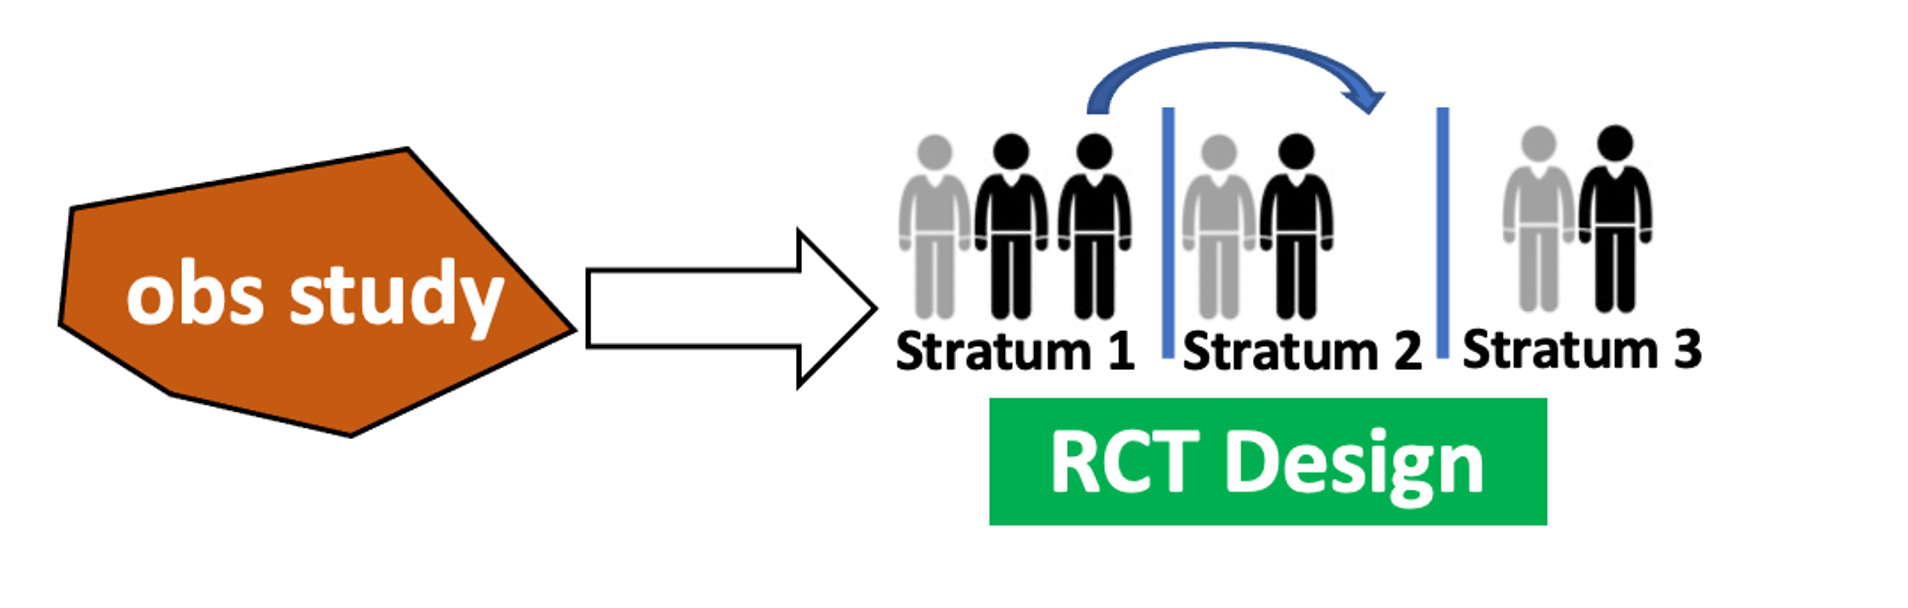
\includegraphics[width = 0.68\textwidth]{Schematic_2}
\end{figure}
\end{frame}


 
\begin{frame}{Estimator and Risk}
We proceed with our estimator $\bskap_{2+}$ from the prior section:
\[ \bskap_{2+} = \htaur - \left\{ \frac{\Tr(\bsSig_r^2 \bsD)\bsSig_r}{(\htauo - \htaur)^\tran  \bsSig_r^2 (\htauo - \htaur) } \right\}_{[0, 1]} \left( \htaur - \htauo \right)\]
\vspace{3mm} \\ \pause
\noindent Optimize experimental design over $\mathcal{R}_2(\boldsymbol{d}, \boldsymbol V, \bsxi)$, the risk of $\bskap_{2+}$ under fixed $\tauo$, with \pause
\begin{itemize}
\item design $\boldsymbol{d}$ \pause
\item stratum potential outcome variances $\boldsymbol V = \{(\hat \sigma_{kt}^2, \hat \sigma_{kc}^2)\}_{k = 1}^K$ \pause
\item bias vector $\bsxi$.
\end{itemize} \pause
\vspace{2mm}
Can compute this efficiently via numerical integration \citep{bao2013moments}, as long as $\boldsymbol V$ and $\bsxi$ are known. 
\end{frame}

\begin{frame}{Design Heuristics}
Can estimate $\boldsymbol{ \hat V}$ using pilot estimates obtained from ODB: 
\begin{align*}
\hat \sigma_{kt}^2 &= \widehat \var \left( Y(1) \mid S = k \right) \hspace{5mm} \text{ and } \hspace{5mm} \hat \sigma_{kc}^2 = \widehat \var \left( Y(0) \mid S = k \right)\,.
\end{align*}\pause

Design heuristics:
\begin{enumerate}
\item \textbf{Na\"ive Optimization}: Assume $\bsxi = 0$ and minimize $\mathcal{R}_2(\boldsymbol{d}, \boldsymbol{ \hat V}, \bsxi = 0)$ over $\boldsymbol{d}$, via \textbf{greedy swap algorithm}. 
\item \textbf{Robust Optimization}: Under model of  \cite{tan2006distributional} and a user-chosen value of sensitivity $\Gamma \geq 1$, optimize the design $\boldsymbol{d}$ under worst-case bias
\end{enumerate}

\end{frame}



\begin{frame}{Acknowledgments}
Thank you to my collaborators on this work: 
\begin{multicols}{2}
\begin{itemize}
\item Guillaume Basse
\item Mike Baiocchi
\item Art Owen
\item Francesca Dominici 
\item Luke Miratrix 
\end{itemize}
\end{multicols}

\vspace{3mm}

Posited shrinkage structure paper available in \color{blue}Biometrics\color{black}\\
Hierarchical model paper (as of Wednesday!) at {\color{blue}arXiv:2204.06687}\\
Design paper available at \color{blue}arXiv:2204.06687\color{black}
\end{frame}

\begin{frame}{Thanks!}

\end{frame}

\begin{frame}[allowframebreaks]{References}
\tiny
\bibliographystyle{apalike} % This yields author(year) citations. 
\bibliography{rct+odb}      % bib for this and related papers 
\normalsize
\end{frame}

\appendix 

\begin{frame}{Appendices}
\end{frame}


\begin{frame}{Practical Considerations}
\begin{itemize}
\item \textbf{Variance estimation:} In practice, $\bsSig_r$ not known. Must be estimated from data.
\vspace{2mm}
\item \textbf{Propensity score adjustment} 
\begin{itemize}
\item No unconfoundedness $\implies$ \\ propensity score adjustment can't remove all bias 
\item If ODB is large, adjusting will typically be good practice. We suggest stabilized IPTW adjustments. 
\end{itemize}
\vspace{2mm}
\item \textbf{Sensitivity analysis}
\begin{itemize}
\item Marginal sensitivity model of \cite{tan2006distributional} summarizes degree of unmeasured confounding by a single value, $\Gamma \geq 1$
\item Can ``reverse engineer" implied confounding value $\Gamma_{\text{imp}}$ when using a shrinker, via work of \cite{zhao2019sensitivity}
\item Evaluate $\Gamma_{\text{imp}}$  to obtain a $\Large \greencheck$ or $\large \color{red} \text{\sffamily X}$ for using shrinker
\end{itemize}
\end{itemize} 
\end{frame}


\begin{frame}{A Note on $\lambda_1^{\URE}$}

The true risk-minimizing shrinkage weight is given by
\[ \lambda_{\text{opt}} = \frac{\Tr(\bsSig_r\bsD)}{\Tr(\bsSig_r\bsD) + \Tr(\bsSig_o \bsD) + \underbrace{\bsxi^\tran \bsD^2 \bsxi}_{\text{Not estimable from data}}} \,,\]
but observe that 
\[ E \left(\left( \htauo - \htaur\right)^\tran \bsD\left( \htauo - \htaur\right) \right) = \Tr(\bsSig_r\bsD) + \Tr(\bsSig_o \bsD) + \bsxi^\tran \bsD^2 \bsxi\,.\] 
$\lambda_1^{\URE} $ substitutes the quadratic form for its expectation, 
\[ \lambda_1^{\URE} =\frac{\Tr(\bsSig_r \bsD)}{\left( \htauo - \htaur\right)^\tran \bsD\left( \htauo - \htaur\right) } \,.\]
\end{frame}





\begin{frame}{Guardrails}

Simplicity of Algorithm \ref{eq:greedyAlg} makes it easy to impose guardrails $\Longrightarrow$ \\
\hspace{5mm} for any invalid design, just set objective value to $\infty$.\\
\vspace{3mm}
Recommend simple guardrails for designs:

\begin{enumerate}
\item \textbf{Sample size}: to retain CLT, enforce 
\[ \min_k n_{rkt} \geq SS_{\text{min}}, \hspace{2mm} \min_k n_{rkc} \geq SS_{\text{min}} \] 
\item  \textbf{Detachability}: for default design $\boldsymbol{\tilde d} =  \{\tilde n_{rkt}, \tilde n_{rkc}\}_k$ and tolerance parameter  $\delta_d \geq 1$, enforce 
\[ \sum_k  \frac{\hat \sigma_{kt}^2}{n_{rkt}'} + \frac{\hat \sigma_{kc}^2}{n_{rkc}'} \geq \delta_d \sum_k  \frac{\hat \sigma_{kt}^2}{\tilde n_{rkt}} + \frac{\hat \sigma_{kc}^2}{\tilde n_{rkc}}\,, \] 
for any proposed design $\boldsymbol{d'} = \{n_{rkt}', n_{rkc}'\}_k$. 
\item \textbf{Risk reduction}: for proposed $\boldsymbol{d'} = \{n_{rkt}', n_{rkc}'\}_k$, enforce
\begin{align*}
4 \max_k & \left( \frac{\hat \sigma_{kt}^2}{n_{rkt}'} + \frac{\hat \sigma_{kc}^2}{n_{rkc}'} \right)^2 >  
 \sum_k \left(  \frac{\hat \sigma_{kt}^2}{n_{rkt}'} + \frac{\hat \sigma_{kc}^2}{n_{rkc}'} \right)^2. 
\end{align*}
This is the condition enforcing that the risk of $\bskap_{2}$ is lower than that of $\taur$. 
\end{enumerate}
\end{frame}


\begin{frame}{Application to the WHI}
\begin{itemize}
\item Split RCT data into ``gold" and ``silver" subsets
\item Gold dataset: used to obtain ``gold standard" estimates of stratum treatment effects
\item Repeat $1,000$ times:
\begin{itemize}
\item Draw bootstrap samples:
\begin{itemize}
\item $1,000$ RCT units (from silver data)
\item Observational sample (50K units)
\end{itemize} 
\item Compute $L_2$ loss for $\htaur, \bskap_{1+}, \bskap_{2+}, \bsdelt_1, \bsdelt_2$. 
\end{itemize}
\item Average loss over draws 
\end{itemize}
\end{frame}

\begin{frame}{Stratification Variables}
Stratify on two variables from WHI protocol  \citep{roehm2015reappraisal}:\\\textbf{Age} $+$ \textbf{CVD} (history of cardiovascular disease) \\
\vspace{5mm}
Also include a variable unassociated with potential outcomes: \\\textbf{Langley} (solar irradiance)

\end{frame}

\begin{frame}{Results}
 \begin{columns}
    \column{\dimexpr\paperwidth-10pt}

% Please add the following required packages to your document preamble:
% \usepackage{multirow}
\begin{table}[]
\begin{tabular}{lllllll}
\hline
\multirow{2}{*}{\textbf{\begin{tabular}[c]{@{}l@{}}Subgroup\\ Variable(s)\end{tabular}}} & \multirow{2}{*}{\textbf{\begin{tabular}[c]{@{}l@{}}\# of \\ Strata\end{tabular}}} & \multirow{2}{*}{\textbf{\begin{tabular}[c]{@{}l@{}}Avg. $\htaur$ \\Loss   \end{tabular}}} & \multicolumn{4}{l}{\textbf{Loss as \% of RCT-Only Loss}}                          \\ \cline{4-7} 
                                                                                         &                                                                                   &                                                                                         &$\bskap_{1+}$ & $\bskap_{2+}$ &$\bsdelt_1$ & $\bsdelt_2$ \\ \hline \\\vspace{0.16cm}
\textbf{Age}                                                                             & 3                                                                                 & 0.00064                                                                                 & 40.1\%               & \textbf{\color{ForestGreen}{34.3\%}}               & 63.3\%           & 74.8\%           \\\vspace{0.16cm}

\textbf{\begin{tabular}[c]{@{}l@{}}Cardiovascular \\ disease (CVD)\end{tabular}}                                                                              & 2                                                                                 & 0.00149                                                                                 & 40.6\%               & \textbf{\color{ForestGreen}{39.6\%}}               & 100\%          & 100\%          \\\vspace{0.2cm}

\textbf{Solar}                                                                         & 5                                                                                 & 0.00094                                                                                 & 29.1\%               & \textbf{\color{ForestGreen}{18.2\%}}               & 43.1\%           & 52.9\%           \\\vspace{0.16cm}

\textbf{Age, CVD}                                                                        & 6                                                                                 & 0.00574                                                                                 & 25.0\%               & \textbf{\color{ForestGreen}{14.0\%}}               & 30.6\%           & 85.6\%           \\\vspace{0.16cm}

\textbf{CVD, Solar}                                                                    & 10                                                                                & 0.00803                                                                                 & \textbf{\color{ForestGreen}{20.9\%}}               & 21.2\%               & 21.0\%           & 88.4\%           \\\vspace{0.16cm}

\textbf{Age, Solar}                                                                    & 15                                                                                & 0.00398                                                                                 & 31.2\%               & 30.4\%               & \textbf{\color{ForestGreen}{28.4\%}}           & 58.4\%           \\\vspace{0.16cm}

\textbf{\begin{tabular}[c]{@{}l@{}}Age, CVD, \\ Solar\end{tabular}}                    & 30                                                                                & 0.02901                                                                                 & 15.8\%               & 16.1\%               & \textbf{\color{ForestGreen}{15.7\%}}           & 88.3\%          
\end{tabular}
\caption{Empirical risk using bootstrap samples of size $1,000$ from RCT data.}

\end{table}
\end{columns}
\end{frame}


\begin{frame}[allowframebreaks]{Simulations Set-Up}
\begin{itemize}
\item ODB has 20K units ($j \in \mathcal{O}$). RCT has 1,000 ($i \in \mathcal{E}$)
%\item For $\ell \in \mathcal{O} \cup \mathcal{E}$, draw $X_{\ell} \simiid \mathcal{N}(0, \boldsymbol I_5)$
\item Untreated potential outcomes $Y_{\ell} \in \{0, 1\}$ for $\ell \in \mathcal{O} \cup \mathcal{E}$ sampled as indep. Bernoullis with
\[\text{Pr}(Y_\ell(0) = 1 \mid \bsx_\ell) = \frac{1}{1 + e^{-\alpha -\beta^\tran\bsx_\ell + \err_\ell}} ,\quad\text{for $\beta = (1,1,1,1,1)^\tran$}\]  
for covariates $X_{\ell} \simiid \mathcal{N}(0, \boldsymbol I_5)$, $\alpha$ chosen s.t. mean is 10\%. 
\item Treatment variables $W_j$ for $j \in \mathcal{O}$ sampled via
\[\text{Pr}(W_j = 1 \mid \bsx_j) = \frac{1}{1 + e^{-\gamma^\tran\bsx_j}},\quad\text{for $\gamma = (\sqrt{2}, \sqrt{2}, \sqrt{2}, 0, 0)^\tran$.}\] 
\pagebreak
\item Treatment effects 
\begin{itemize}
\item Define $k = 1, \dots, 12$ strata based on first $+$ second covariate 
\item Assign $\tau_k$,  stratum CATEs, via 3 treatment effect models:
\[ \tau_k  = T, \quad \tau_k = -T\times \frac{k}{K},\quad\text{and}\quad
\tau_k  = T\times \left(\frac{k}{K}\right)^2 \] 
\item  $T$ chosen so that Cohen's D in ODB equals 0.5 
%\item Choose $\tau_k \times n_k$ units for which $Y_{\ell}(0) = 0$, and set $Y_{\ell}(1) = 1$. For remaining units, $Y_{\ell}(0) = Y_{\ell}(1)$
\end{itemize}
\item Simulation structure
\begin{itemize}
\item Sample ODB data a single time. Correct via SIPW.  
\item Compute RCT designs under different heuristics 
\item Resample RCT units $5,000$ times. For each sample, compute $L_2$ error in estimating $\bstau$ using $\taur, \bskap_2,$ and $\bskap_{2+}$
\end{itemize}
\end{itemize}
\end{frame}

\begin{frame}{Idealized Case: All Covariates Measured} 
\small

\begin{table}[h]
\centering
\begin{tabular}{ll|rrr|rrrr|r}
\toprule
 & & & & &  \multicolumn{4}{c|}{\textbf{Max Bias, }$\boldsymbol \Gamma$ \textbf{Value} } &  \\ 
\textbf{Est}  & \textbf{Trt}    & \textbf{Eq.} & \textbf{Ney.} & \textbf{Naïve} & \textbf{1.0} & \textbf{1.1} & \textbf{1.2} & \textbf{1.5} & \textbf{Oracle} \\ \midrule
$\taur$   & \multirow{3}{*}{c} & 100\% & \textbf{\color{ForestGreen}{87\%}} & 91\% & 100\% & 96\% & 94\% & 94\% & 96\% \\
$\bskap_2$      &  & 82\% & 48\% & \textbf{\color{ForestGreen}{44\%}} & 52\% & 48\% & 47\% & 50\% & 42\% \\
$\bskap_{2+}$ & &38\% & 28\% & \textbf{\color{ForestGreen}{26\%}} & 26\% & 26\% & 26\% & 28\% & 23\% \\ \midrule
$\taur$   &  \multirow{3}{*}{$\ell$} & 100\% & \textbf{\color{ForestGreen}{89\%}} & 92\% & 95\% & 94\% & 95\% & 97\% & 104\% \\
$\bskap_2$      &  & 93\% & 66\% & 58\% & 58\% & \textbf{\color{ForestGreen}{57\%}} & 60\% & 64\% & 50\% \\
$\bskap_{2+}$ & & 59\% & 51\% & 45\% & \textbf{\color{ForestGreen}{43\%}} & 45\% & 47\% & 49\% & 33\% \\ \midrule				
$\taur$   & \multirow{3}{*}{q} & 100\% & \textbf{\color{ForestGreen}{86\%}} & 91\% & 95\% & 98\% & 94\% & 92\% & 91\% \\
$\bskap_{2}$  & &81\% & 47\% & \textbf{\color{ForestGreen}{45\%}} & 52\% & 52\% & 50\% & 48\% & 41\% \\
$\bskap_{2+}$ & & 37\% & 29\% & \textbf{\color{ForestGreen}{27\%}} & 28\% & 28\% & 30\% & 29\% & 25\% \\ \bottomrule
 \end{tabular} 
\caption{\label{tab:idealized} Risk over $5,000$ iterations of $\taur, \bskap_2$, and $\bskap_{2+}$ in the case of no unmeasured confounding in the observational study. Risks are expressed as a percentage of the risk of $\taur$ using an equally allocated experiment, for each of the three treatment effect models.}
\end{table}\end{frame}


\begin{frame}{Realistic Case: Third Covariate Missing}
\small
\begin{table}[h]
\centering
\begin{tabular}{ll|rrr|rrrr|r}
\toprule
 & & & & &  \multicolumn{4}{c|}{\textbf{Max Bias, }$\boldsymbol \Gamma$ \textbf{Value} } &  \\ 
\textbf{Est}  & \textbf{Trt}    & \textbf{Eq.} & \textbf{Ney.} & \textbf{Naïve} & \textbf{1.0} & \textbf{1.1} & \textbf{1.2} & \textbf{1.5} & \textbf{Oracle} \\ \midrule
$\taur$   & \multirow{3}{*}{c}& 100\% & \textbf{\color{ForestGreen}{90\%}} & 90\% & 90\% & 92\% & 93\% & 95\% & 102\% \\
$\bskap_2$      &  &102\% & 81\% & 74\% & \textbf{\color{ForestGreen}{72\%}} & 72\% & 72\% & 77\% & 69\% \\
$\bskap_{2+}$      &  &96\% & 80\% & 74\% & \textbf{\color{ForestGreen}{71\%}} & 72\% & 72\% & 76\% & 67\% \\ \midrule
$\taur$   & \multirow{3}{*}{$\ell$} & 100\% & 93\% & \textbf{\color{ForestGreen}{93\%}} & 94\% & 95\% & 96\% & 96\% & 104\% \\
$\bskap_2$      & &102\% & 85\% & 77\% & \textbf{\color{ForestGreen}{75\%}} & 76\% & 77\% & 79\% & 73\% \\
$\bskap_{2+}$ & & 98\% & 84\% & 77\% & \textbf{\color{ForestGreen}{75\%}} & 76\% & 76\% & 79\% & 71\% \\ \midrule
$\taur$   & \multirow{3}{*}{q} &100\% & \textbf{\color{ForestGreen}{89\%}} & 90\% & 93\% & 92\% & 91\% & 96\% & 96\% \\
$\bskap_{2}$ & &101\% & 74\% & 69\% & 68\% & 68\% & \textbf{\color{ForestGreen}{67\%}} & 73\% & 66\% \\ 
$\bskap_{2+}$ & &88\% & 72\% & 67\% & 66\% & 66\% & \textbf{\color{ForestGreen}{65\%}} & 71\% & 63\% \\ \bottomrule
 \end{tabular} 
\caption{\label{tab:practical} Risk over $5,000$ iterations of $\taur, \bskap_2$, and $\bskap_{2+}$ under various experimental designs, in the case of unmeasured confounding in the observational study via failure to measure the third covariate.}
\end{table} 
\end{frame}


\begin{frame}{1. Neyman Allocation}

Using stronger form of Assumption 3 (shared variances), we can estimate from the ODB: 
\begin{align*}
\hat \sigma_{kt}^2 &= \widehat \var \left( Y(1) \mid S = k \right) \hspace{5mm} \text{ and } \hspace{5mm} \hat \sigma_{kc}^2 = \widehat \var \left( Y(0) \mid S = k \right) \,. 
\end{align*} 

Simplest design heuristic: use a Neyman allocation without a cost constraint, e.g. 
\begin{align*}
n_{rkt} = \frac{n_r \cdot\hat \sigma_{kt}^2}{\sum_k\hat \sigma_{kt}^2 +  \hat \sigma_{kc}^2}\ \hspace{5mm} \text{ and } \hspace{5mm} n_{rkc} &= \frac{n_r \cdot \hat \sigma_{kc}^2}{\sum_k\hat \sigma_{kt}^2 +\hat \sigma_{kc}^2}\,.
\end{align*}

Optimizes over only the non-shrinkage portion of the risk, but reasonable in many practical settings. 

\end{frame}


\begin{frame}{Improving Interpretability of $\bskap_{1+}$}
\begin{itemize}
\item Recall: $\lambda_1^{\URE}$ can be interpreted as an estimate of 
\[ \lambda_{\text{opt}} = \frac{\Tr(\bsSig_r\bsD)}{\Tr(\bsSig_r\bsD) + \Tr(\bsSig_o \bsD) + \bsxi^\tran \bsD^2 \bsxi}\,, \]
true MSE-minimizing weight on $\htauo$ in a convex combination
\item We can use this idea to improve interpretability of $\bskap_{1+}$!
\item \textbf{Key idea}:  frame in context of sensitivity model of \cite{tan2006distributional}
\end{itemize}
\end{frame}

\begin{frame}{Prior Work}
\begin{itemize}
\item Marginal sensitivity model of \cite{tan2006distributional} summarizes degree of unmeasured confounding by a single value, $\Gamma \geq 1$
\begin{itemize}
\item $\Gamma$ bounds odds ratio of treatment prob. conditional on potential outcomes + covariates vs. covariates only
\item Related to the famous model of \cite{rosenbaum1987sensitivity}, but extends to the setting of inverse probability weighting 
\end{itemize}
\item \cite{zhao2019sensitivity} derive valid confidence intervals for causal estimates under the set of models indexed by any choice of $\Gamma$
\begin{itemize}
\item Implicitly maps $\Gamma$ to a worst-case bias $\xi(\Gamma)$ and variance $\Sigma_O(\Gamma)$
\item Under some assumptions, allows us to obtain worst-case estimate of $\lambda_{\text{opt}}$ as a function of $\Gamma$, which we call $\lambda(\Gamma)$
\end{itemize}
\end{itemize}
\end{frame}



\begin{frame}{Relating the Models}
\begin{itemize}
\item \textbf{Intuition}: larger $\Gamma$ (confounding parameter) $\implies$ optimal weight $\lambda_{\text{opt}}$ is smaller 
\item Let  $\Gamma_{\text{imp}} = \sup \{\Gamma: \lambda(\Gamma) > \lambda_1^{\URE}\}$
\begin{itemize}
\item Largest value $\Gamma$ for which the optimal shrinkage factor $\lambda(\Gamma)$ is greater than our shrinkage parameter $\lambda_1^{\URE}$. 
\end{itemize}
\item $\Gamma_{\text{imp}} $ can be used to evaluate level of shrinkage 
\begin{itemize}
\item If we believe true confounding level $\Gamma < \Gamma_{\text{imp}}$, then
\[ \lambda_1^{\URE} \approx \lambda(\Gamma_{\text{imp}}) \leq \lambda_{\text{opt}} = \lambda(\Gamma) \] 
Hence the shrinkage level is conservative. $\Large \greencheck$
\item If we believe  $\Gamma > \Gamma_{\text{imp}}$, then estimator is overshrinking, relies too much on the observational estimate. $\large  \color{red} \text{\sffamily X}$
\end{itemize}
\end{itemize}
\end{frame}


\begin{frame}[allowframebreaks]{1. Na\"ive Optimization Assuming $\bsxi \boldsymbol{= 0}$}

Using stronger Assumption 3 (shared var), can estimate from ODB: 
\begin{align*}
\hat \sigma_{kt}^2 &= \widehat \var \left( Y(1) \mid S = k \right) \hspace{5mm} \text{ and } \hspace{5mm} \hat \sigma_{kc}^2 = \widehat \var \left( Y(0) \mid S = k \right)\,. 
\end{align*} 

Define $\mathcal{R}_2(\boldsymbol{d}, \boldsymbol V, \bsxi) = \mathcal{R}(\bskap_2)$ analyzed under design $\boldsymbol{d}$, potential outcome variances $\boldsymbol V = \{(\hat \sigma_{kt}^2, \hat \sigma_{kt}^2)\}_{k = 1}^K$, and error $\bsxi$. \\ 
\vspace{3mm}
Simple heuristic: assume $\bsxi = 0$. Then solve:

\begin{equation}\label{optProb:riskExpNoConfound}
\begin{aligned}
\text{ minimize} & \hspace{5mm} \mathcal{R}_2(\boldsymbol{d}, \boldsymbol V, \bsxi) \\
\text{ subject to} & \hspace{5mm} \bsxi = 0, \boldsymbol{V} = \{ ( \hat \sigma_{kt}^2, \hat \sigma_{kc}^2 ) \}_{k = 1}^K, \\
%\sigma_{rk}^2 = \frac{\hat \sigma_{kt}^2}{n_{rkt}} + \frac{\hat \sigma_{kc}^2}{n_{rkc}}, \hspace{2mm} k = 1, \dots, K, \\
& \hspace{5mm} 0 < n_{rkt}, n_{rkc}, , \hspace{2mm} k = 1, \dots, K, \\
& \hspace{5mm}n_r = \sum_k n_{rkt} + n_{rkc}\,.
\end{aligned}
\end{equation} 

But $\mathcal{R}_2(\boldsymbol{d}, \boldsymbol V, \bsxi)  $ is not convex in the design $\boldsymbol{d}$... 
\pagebreak

A practical approach: \textbf{greedy algorithm}. 
Define $\boldsymbol{d_j}$ as design on $j^{th}$ iteration, and define 
\[ \mathcal{D}_j = \{ \boldsymbol d' \mid \text{ $\boldsymbol d'$ changes one unit across strata/treatment level from } \boldsymbol{d}_j \}\,. \] 
Run Algorithm \ref{eq:greedyAlg} from several values of $\boldsymbol{d}_0$ and take minimum:

\small
\begin{equation}\label{eq:greedyAlg}
\begin{split}
& \texttt{Start with design $\boldsymbol{d_0} = \{ (n_{rkt}^{(0)}, n_{rkc}^{(0)})\}_k$.} \hspace{25mm} \\
& \texttt{For iteration $j = 1, 2, \dots$:}\\
& \hspace{5mm} \texttt{For each design $\boldsymbol d'$ in $\mathcal{D}_{j-1}$:}\\
& \hspace{10mm} \texttt{Compute $\mathcal{R}_2(\boldsymbol{d'}, \boldsymbol V, 0) )$. } \\
& \hspace{5mm} \texttt{Set $\boldsymbol{d_j} = \argmin_{\boldsymbol{d'} \in \mathcal{D}_{j - 1}} \mathcal{R}_2(\boldsymbol{d'}, \boldsymbol V, 0) $} \\
& \hspace{5mm} \texttt{If $\mathcal{R}_2(\boldsymbol{d_j}, \boldsymbol V, 0)  >=  \mathcal{R}_2(\boldsymbol{d_{j-1}}, \boldsymbol V, 0) $}\\
& \hspace{10mm} \texttt{Return $d_{j - 1}.$}\\
\end{split}
\end{equation}
\end{frame}


\begin{frame}{Designs}
\hspace{-5mm}
\begin{figure}
\centering
\includegraphics[width = 1.05\textwidth]{Allocations.png}
\caption{Allocations of $n_r = 1,000$ units in WHI with strata defined by history of CVD and age, under different design heuristics.}
\end{figure}
\end{frame}


\begin{frame}{Simulated Data Visualization}
\begin{figure}
\centering
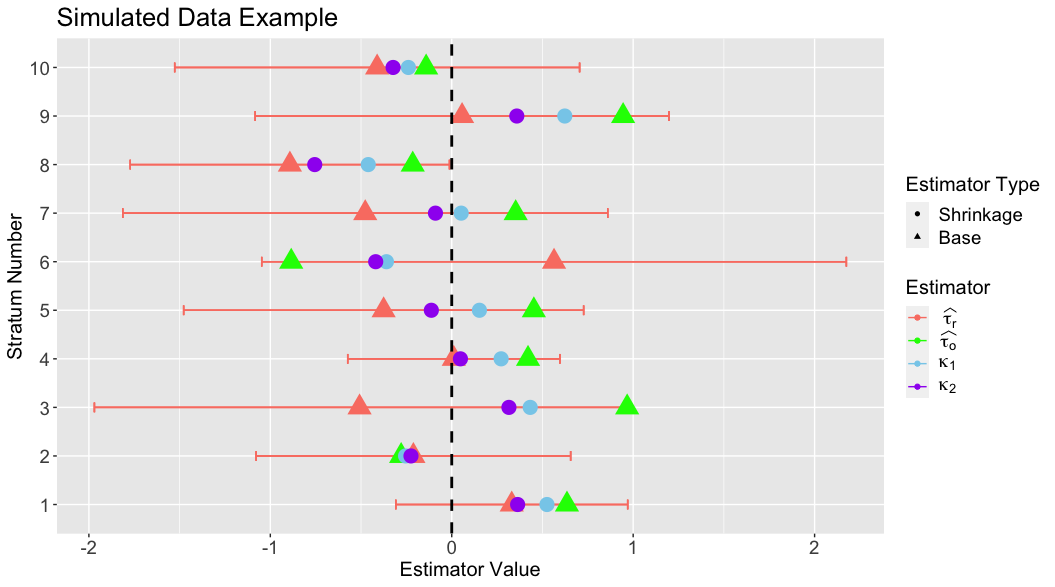
\includegraphics[width =1.\textwidth]{Simulated_Visuals_v2}
\caption{Simulated shrinkage between \color{red}$\htaur$ \color{black} and \color{green}$\htauo$ \color{black} with ten strata. 90\% conf. sets for  \color{red}$\htaur$ \color{black} in  \color{red}red\color{black}, with \color{cyan}$\bskap_{1+}$ \color{black} and \color{darkorchid}$\bskap_{2+}$ \color{black} shown in circles. }
\end{figure}
\end{frame}


\begin{frame}{1. Na\"ive Optimization Assuming $\bsxi \boldsymbol{= 0}$}

Under enhanced transportability assumption, can estimate $\boldsymbol{ \hat V}$ using pilot estimates obtained from ODB: 
\begin{align*}
\hat \sigma_{kt}^2 &= \widehat \var \left( Y(1) \mid S = k \right) \hspace{5mm} \text{ and } \hspace{5mm} \hat \sigma_{kc}^2 = \widehat \var \left( Y(0) \mid S = k \right)\,.
\end{align*}\pause
\vspace{5mm}\\
Use a simple heuristic: assume $\bsxi = 0$.\\
\vspace{5mm}
Minimize $\mathcal{R}_2(\boldsymbol{d}, \boldsymbol{ \hat V}, \bsxi = 0)$ over $\boldsymbol{d}$, via \textbf{greedy swap algorithm}. 
\begin{itemize}
\item Swap units across strata, treatment statuses until no improvement in $\mathcal{R}_2(\boldsymbol{d}, \boldsymbol{ \hat V}, 0)$
\item Non-convexity: run from several starting points. 
\end{itemize}

\end{frame}

\begin{frame}{2. Heuristic Optimization Assuming Worst-Case Error Under $\boldsymbol \Gamma$-Level Unmeasured Confounding}

\begin{itemize}
\item Can take a more pessimistic approach using marginal sensitivity model of \cite{tan2006distributional} 
\item For a user-chosen value of $\Gamma \geq 1$: 
\begin{itemize}
\item can obtain worst-case $\xi_k(\Gamma)$ using  \cite{zhao2019sensitivity}, and...
\item can obtain associated $\hat \sigma_{kt}^2$ and $\hat \sigma_{kc}^2$. \\
\end{itemize}
\end{itemize} \pause
\vspace{5mm}
posit a value of $\Gamma$ $\Longrightarrow$ \\
\hspace{3mm} collect results into  $\boldsymbol V_{\Gamma}$ and $\bsxi_{\Gamma}$$\Longrightarrow$   \\
\hspace{6mm} run greedy algorithm on $\mathcal{R}_2(\boldsymbol d, \boldsymbol V_{\Gamma}, \bsxi_{\Gamma})$ instead of $\mathcal{R}_2(\boldsymbol d, \boldsymbol{ \hat V}, 0)$
\end{frame}



\end{document}
